%%%%%%%%%%%%%%%%%%%%%%%%%%%%%%%%%%%%%%%%%%%%%%%%%%%%%%%%%%%%%%%%%%%%%%%%%
%           Capítulo 2: MARCO TEÓRICO - REVISIÓN DE LITERATURA
%%%%%%%%%%%%%%%%%%%%%%%%%%%%%%%%%%%%%%%%%%%%%%%%%%%%%%%%%%%%%%%%%%%%%%%%%

\chapter{Teor\'ia}
Consideremos un mapeo $M$ que preserva \'area, donde $M:\mathbb{S} \times \mathbb{R} \longrightarrow \mathbb{S}\times\mathbb{R}$. El mapeo $M$ lleva puntos $v_{i}= (x_{i},y_{i})$ en puntos dados por $M(v_{i})=v_{i+1}$, donde el sub\'indice denota que se trata de la i-\'esima iteraci\'on. \\

Nos interesa centrarnos en los mapeos que violan la condici\'on de no degeneraci\'on tambi\'en llamada \textit{condici\'on twist} que dice que 
\begin{eqnarray}
\frac{\partial x_{i+1}}{\partial y_{i}} \neq 0.
\label{twist condition}
\end{eqnarray}
Un mapeo puede violar la condici\'on \ref{twist condition} de diferentes maneras, en especial si para alg\'un valor particular de $y_{i}$ ocurre que $\partial x_{i+1}/\partial y_{i} = 0$. La violaci\'on de la condici\'on \ref{twist condition} da lugar a bifurcaciones de los c\'irculos invariantes, las cuales a su vez son indicadoras de una colisi\'on de \'orbitas peri\'odicas en el mapeo. El valor del par\'ametro para el cual ocurre la colisi\'on es de importancia en teor\'ia KAM. 

\section{Un m\'etodo para encontrar \'orbitas peri\'odicas de mapeos de 2D.}

Los m\'etodos para encontrar \'orbitas peri\'odicas en mapeos de dos dimensiones son generalmente m\'etodos para encontrar ra\'ices de sistemas no lineales en dos dimensiones. En este caso se busca reducir la dimensi\'on en la que se trabaja para encontrar \'orbitas per\'iodicas. Para ello es necesario encontrar algunas simetr\'ias que reduzcan el problema a una dimensi\'on. Veremos que las \'orbitas peri\'odicas se pueden encontrar usando simetr\'ias e involuciones.\\

Decimos que el mapeo $M$ permanece invariante bajo un mapeo $T$ o que conmuta con $T$ si 
\begin{eqnarray}
TM = MT,
\label{conmuta}
\end{eqnarray}
esta carater\'istica nos ayudar\'a a redefinir una \'orbita peri\'odica del mapeo. Por otro lado decimos que una transformaci\'on $I$ se dice de \textit{tiempo inverso} para $M$ si 
\begin{eqnarray}
I_{0}M^{-1} = MI_{0}.
\label{involucion1}
\end{eqnarray}
Es decir si la simetr\'ia cambia el sentido del mapeo hac\'ia atr\'as. Si adem\'as la simetr\'ia de tiempo inverso es una involuci\'on ($I_{0}^{2}=1$) se puede construir una nueva involuci\'on a partir de la anterior mediante 
\begin{equation}
I_{1} = MI_{0}.
\label{involucion2}
\end{equation}
Es simple comprobar que $I_{1}$ es involuci\'on, usando la definici\'on \ref{involucion1} tenemos que 
\begin{equation*}
I_{1}^{-1}MI_{1} = (MI_{0})^{-1}MI_{1} = I_{0}^{-1}M^{-1}MI_{1} = I_{0}^{-1}I_{1} = I^{-1}_{0}MI_{0}=M^{-1},
\end{equation*}
y reacomodando t\'erminos obtenemos $I_{0}M^{-1}= MI_{0}$.\\

 
Con las involuciones definidas arriba podemos escribir el mapeo $M$ como factorizaci\'on de las mismas
\begin{eqnarray}
M = I_{1}I_{0}.
\end{eqnarray}
Decimos entonces que el mapeo $M$ es reversible. Usando estos conceptos vamos a analizar la siguiente afirmaci\'on. \\

\begin{thm}
Sea $M:\mathbb{S} \times \mathbb{R} \longrightarrow \mathbb{S}\times\mathbb{R}$ un mapeo simpl\'ectico no-twist reversible. Sean 
\begin{eqnarray}
\mathbb{J}_{0} = \{v \in \mathbb{S} \times \mathbb{R} | I_{0}v = v\}
\end{eqnarray}
\begin{eqnarray}
\mathbb{J}_{1} = \{v \in \mathbb{S} \times \mathbb{R} | I_{1}v = v\}
\end{eqnarray}
Si $v_{0}\in \mathbb{J}_{0}$ y $M^{N}v_{0}=v_{N}\in \mathbb{J}_{0}$ entonces $v_{0}$ es de periodo $2N$.
\end{thm}
\textit{Demostraci\'on:}\\
Queremos probar que $M^{2N}v_{0}=v_{0}$. Entonces
\begin{align*}
	M^{2N}v_{0} &= M^{N}M^{N}v_{0}\\
				&= M^{N-1}MM^{N-1}Mv_{0}\\
				&= M^{N-1}MM^{N-1}I_{1}I_{0}v_{0},
\end{align*}
usando que $v_{0}\in I_{0}$ y que $M$ es reversible
\begin{align*}
	M^{2N}v_{0} &= M^{N-1}I_{1}I_{0}M^{N-1}I_{1}v_{0},
\end{align*}
usando que $M^{N}v_{0}=v_{N}\in \mathbb{J}_{0}$ y que $M^{N-1}=M^{N}M^{-1}$
\begin{align*}
	M^{2N}v_{0} &= M^{N-1}I_{1}I_{0}M^{N}M^{-1}I_{1}v_{0}\\
				&= M^{N-1}I_{1}	M^{N-1}I_{1}v_{0}.
\end{align*}
Usando que el mapeo es reversible es f\'acil ver que se cumple que
\begin{equation}
I_{1}M=I_{0}
\label{reversible1}
\end{equation}
\begin{equation}
MI_{0} = I_{1}.
\label{reversible2}
\end{equation}
Tomando en cuenta la ecuaci\'on \ref{reversible1}
\begin{align*}
M^{2N}v_{0} &= M^{N-2}MI_{1}MM^{N-2}I_{1}v_{0} \\
			&= M^{N-2}MI_{0}M^{N-2}I_{1}v_{0}\\
			&= M^{N-2}I_{1}M^{N-2}I_{1}v_{0}.
\end{align*}
Usando de nuevo las ecuaciones \ref{reversible1},\ref{reversible2},
\begin{align*}
M^{2N}v_{0} &= M^{N-3}MI_{1}MM^{N-3}I_{1}v_{0} \\
			&= M^{N-3}MI_{0}M^{N-3}I_{1}v_{0}\\
			&= M^{N-3}I_{1}M^{N-3}I_{1}v_{0}.
\end{align*}
De manera sucesiva aplicando \ref{reversible1},\ref{reversible2} obtenemos que 
\begin{align*}
		M^{2N}v_{0}=MI_{1}MI_{1}v_{0},
\end{align*} 
donde por \'ultima vez aplicamos \ref{reversible1} y que $M$ es reversible
\begin{align*}
M^{2N}v_{0}&=MI_{0}I_{1}v_{0}\\
			&= I_{1}I_{0}I_{0}I_{1}v_{0}\\
			&=v_{0}
\end{align*}
De manera an\'aloga se puede demostrar el teorema para $v_{0}\in \mathbb{J}_{1}$.\\

En el caso en que tengamos una \'orbita de periodo impar afirmamos el siguiente teorema. 

\begin{thm}
	Sea $M:\mathbb{S} \times \mathbb{R} \longrightarrow \mathbb{S}\times\mathbb{R}$ un mapeo simpl\'ectico no-twist reversible. Sean 
	\begin{eqnarray}
	\mathbb{J}_{0} = \{v \in \mathbb{S} \times \mathbb{R} | I_{0}v = v\}
	\end{eqnarray}
	\begin{eqnarray}
	\mathbb{J}_{1} = \{v \in \mathbb{S} \times \mathbb{R} | I_{1}v = v\}
	\end{eqnarray}
	Si $v_{0}\in \mathbb{J}_{1}$ y $M^{N}v_{0}=v_{N}\in \mathbb{J}_{0}$ entonces $v_{0}$ es de periodo $2N+1$.
\end{thm}

\textit{Demostraci\'on:}\\
Queremos ver que $M^{2N+1}v_{0}=v_{0}$.\\
Entonces
\begin{align*}
M^{2N+1}v_{0} &= M^{2N}Mv_{0}\\
			&= M^{N}MM^{N}v_{0}.
\end{align*}
Usando que el mapeo es reversible y que $I_{0}M^{N}=M^{N}$,
\begin{align*}
M^{2N+1}v_{0} &= M^{N}I_{1}I_{0}M^{N}v_{0}\\
				&= M^{N}I_{1}M^{N}v_{0}\\
				&= M^{N-1}MI_{1}MM^{N-1}v_{0}.
\end{align*}
Usando \ref{reversible2} y \ref{reversible1},
\begin{align*}
M^{2N+1}v_{0} &= M^{N-1}MI_{0}M^{N-1}v_{0}\\
				&= M^{N-1}I_{1}M^{N-1}v_{0}.
\end{align*}
De manera sucesiva se puede usar \ref{reversible1} y \ref{reversible2} hasta llegar a 
\begin{align*}
M^{2N+1}v_{0} &= MI_{1}M^v_{0}\\
			&= MI_{0}v_{0}\\
			&= I_{1}v_{0}.
\end{align*}
Debido a que $v_{0}\in \mathbb{J}_{1}$ 
\begin{align*}
M^{2N+1}v_{0} = v_{0}.
\end{align*}

En el caso en que $v_{0}\in \mathbb{J}_{0}$ y que $v_{N}\in\mathbb{J}_{1}$ se tiene que $M^{2N-1}v_{0}=v_{0}$ y la demostraci\'on es an\'aloga. \\

Con los teoremas 1 y 2 podemos enunciar el siguiente resultado.

\begin{corola}
		Sea $M:\mathbb{S} \times \mathbb{R} \longrightarrow \mathbb{S}\times\mathbb{R}$ un mapeo simpl\'ectico no-twist reversible y $\mathbb{J}_{0}, \mathbb{J}_{1}$ como se definieron en los teoremas 1 y 2. 
		\begin{itemize}
			\item Si $v_{0}\in \mathbb{J}_{0}$ y $M^{N}v_{0}\in \mathbb{J}_{0}$ si y s\'olo si $v_{0}$ pertenece a una \'orbita de periodo $2N$ de $M$.
			\item Si $v_{0}\in \mathbb{J}_{1}$ y $M^{N}v_{0}\in \mathbb{J}_{1}$ si y s\'olo si $v_{0}$ pertenece a una \'orbita de periodo $2N$ de $M$.
			\item Si $v_{0}\in \mathbb{J}_{1}$ y $M^{N}v_{0}\in \mathbb{J}_{0}$ si y s\'olo si $v_{0}$ pertenece a una \'orbita de periodo $2N+1$ de $M$.
			\item Si $v_{0}\in \mathbb{J}_{0}$ y $M^{N}v_{0}\in \mathbb{J}_{1}$ si y s\'olo si $v_{0}$ pertenece a una \'orbita de periodo $2N-1$ de $M$.
		\end{itemize}
\end{corola}
Si se conocen los conjuntos $\mathbb{J}_{0}, \mathbb{J}_{1}$ entonces la b\'usqueda de \'orbitas peri\'odicas se puede reducir a un b\'usqueda en una dimensi\'on, ya que sabemos que al menos un punto de la \'orbita estar\'an en alguno de los conjuntos.









\section{Método de parametrización}
 Esta sección tiene como objetivo describir el método de parametrización desarrollado por X. Cabré, E. Fontich y R. de la Llave \cite{Haro}. El método fue desarrollado de manera general para conjuntos invariantes, estables e inestables, en puntos hiperbólicos, tratándose de un método semianalítico, es decir parte computacional y parte analítica. El m\'etodo busca describir las variedades usando series.\\
	
%A David no le gusto esto:
%Para ahondar en el método recordemos que anteriormente mencionamos que los conjuntos \eqref{variedad estable}, \eqref{variedad inestable} son conjuntos invariantes. Por otro lado también recordemos la definición de sistema dinámico que nos dice que se trata de un semigrupo actuando sobre un espacio $M$, la manera en la que se genera el sistema es con un difeomorfismo 

Supongamos que $v_{*}\in\mathbb{S} \times \mathbb{R}$ es un punto fijo hiperb\'olico del mapeo $M$. Asociado a $v_{*}$ se tienen dos conjuntos invariantes 
\begin{eqnarray}
\mathbb{W}^{s}=\lbrace v : M^{n}v\rightarrow v_{*} \quad \mathrm{cuando} \quad n\rightarrow \infty \rbrace
\label{variedad estable}
\end{eqnarray}

\begin{eqnarray}
\mathbb{W}^{u}=\lbrace v : M^{n}v\rightarrow v_{*} \quad \mathrm{cuando} \quad n\rightarrow -\infty \rbrace
\label{variedad inestable},
\end{eqnarray}
llamados \textit{variedades estable} e \textit{inestable} respectivamente. \\

Para describir los conjuntos invariantes tomemos  $U\subset \mathbb{W}^{z}$ con $z\in \{u,s\}$ y un abierto $\Theta \subset \mathbb{R}$. Como $U$ es parte de conjunto ivariante entonces
\begin{equation}
M : U\subset \mathbb{W}^{z} \longrightarrow  U\subset \mathbb{W}^{z}.
\end{equation}
Por otro lado podemos encontrar $\mathcal{P}:\mathbb{R}\longrightarrow\mathbb{S} \times \mathbb{R}$ parametrizaci\'on tal que el siguiente diagrama conmute
\begin{eqnarray}
\xymatrix{
	\Theta\subset\mathbb{R} \ar[d]^{\mathcal{P}} \ar[r]^{g} & \Theta\subset\mathbb{R} \ar[d]^{\mathcal{P}} \\
	U\subset\mathbb{R}^{2} \ar[r]^{M} & U\subset\mathbb{R}^{2}
}\label{conmutativo}
\end{eqnarray}
La funci\'on $g$ contiene la dinámica del mapeo pero sobre $\Theta$. A partir del diagrama \ref{conmutativo} obtenemos la siguiente ecuaci\'on de cohomolog\'ia. 

\begin{eqnarray}
M \circ \mathcal{P} =\mathcal{P}  \circ g,  \label{Ecua de invariancia}.
\end{eqnarray}
Una forma gr\'afica de ver lo que nos dice la ecuaci\'on \ref{Ecua de invariancia} es medainte la figura 
\ref{diagrama-conmutativo}.

\begin{figure}[h!]
	\centering
	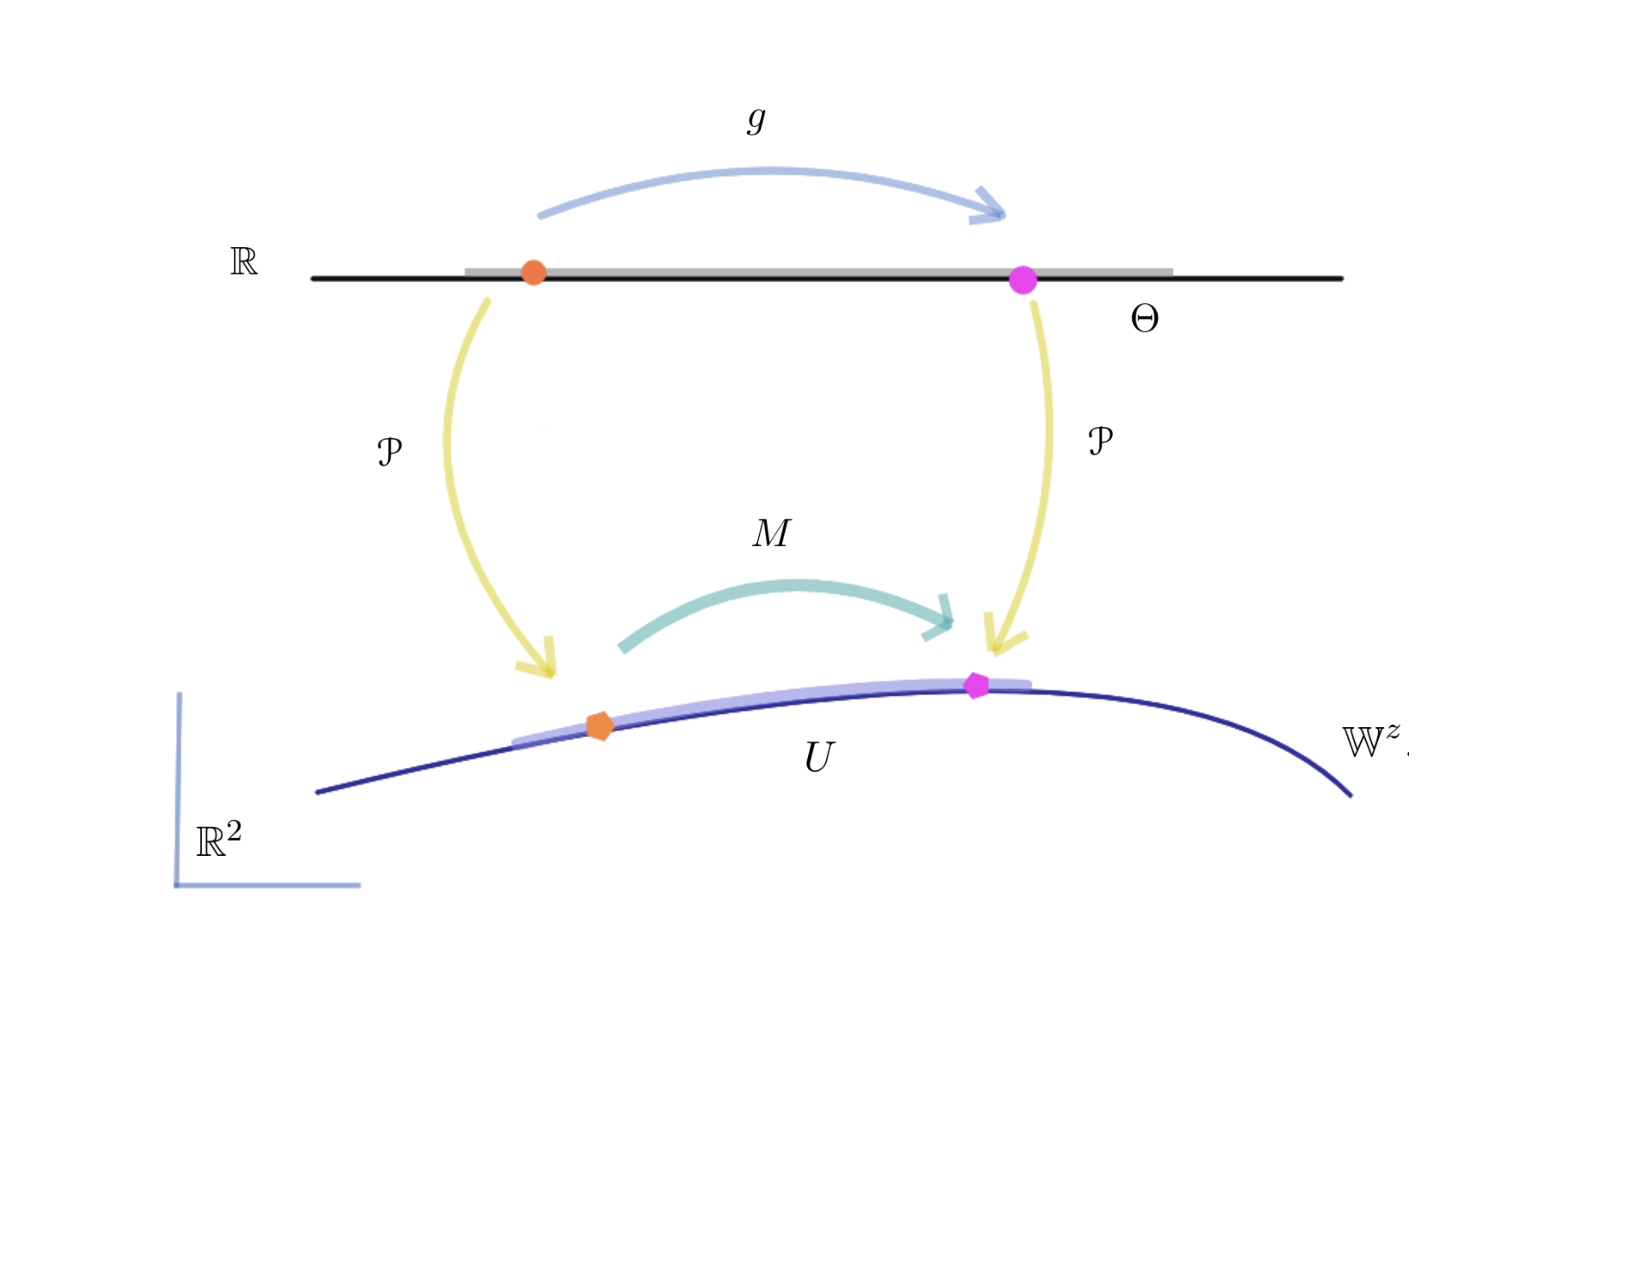
\includegraphics[scale=0.4]{diagrama2}
	\caption{Representación grafica del diagrama \eqref{conmutativo}.}
	\label{diagrama-conmutativo}
\end{figure}

Las variables a encontrar en la ecuaci\'on \ref{Ecua de invariancia} son $\mathcal{P}$ y $g$, por lo que se necesita al menos fijar o encontrar una de ellas para poder resolver la ecuaci\'on. Para hacer esto se suelen tomar en cuenta dos formas de parametrizaci\'on definidas como \textit{la forma gr\'afica} y \textit{la forma normal}. En este caso se usa la forma gr\'afica que consiste en usar la forma local de las variedades al rededor del punto $v_{*}$. Es decir se usa que localmente la dependencia es lineal, por lo que 
\begin{equation}
g(t) = \lambda t,
\label{funciong1}
\end{equation}
con $t\in \mathbb{R}$ el par\'ametro, $\lambda\in \mathbb{R}$ el valor propio asociado a la linearizaci\'on del mapeo. Esta desici\'on esta apoyada en el teorema de Hartman-Grobman que declara que en una vecindad del punto fijo hiperb\'olico se puede aproximar el comportamiento del sistema mediante su linearizaci\'on. \\

Entonces usando la linearizaci\'on del mapeo y la ecuaci\'on \eqref{funciong1} se puede resolver la ecuaci\'on \eqref{Ecua de invariancia} para $\mathcal{P}$. Para ello se propone que 
\begin{equation}
\mathcal{P} := (p_{1}(t), p_{2}(t)) =( \sum_{n=0}^{\infty}a_{n}t^{n}, \sum_{n=0}^{\infty}b_{n}t^{n}).
\label{polinomioecuacion}
\end{equation}
Sustituyendo la ecuaci\'on \eqref{polinomioecuacion} en la ecuaci\'on \eqref{Ecua de invariancia} se puede separar por grado de cada lado de la ecuaci\'on y comparar t\'erminos.  Las ecuaciones resultantes son recursivas , es decir que proponiendo los coeficientes de orden cero del polinomio $\mathcal{P}$ se puede obtener todos los consecutivos. 


